% schem_alg2: Algorithm 2 (per-protocol comparison), column figure.
% Final size 3.30 x 2.80 in (canvas 3.286 x 2.786 in plus a 0.5 pt border),
% included at 100% (width=\linewidth).
% Coordinates in inches from the bottom-left corner of the canvas.
% Interval positions in panel (b) are position only (never printed), from
% results/algo2_reported/pairwise.csv, columns gap/lower/upper_protocol_0
% (zero-shot) and gap/lower/upper_protocol_1 (two-shot), times 100.
% Build: pdflatex -interaction=nonstopmode -halt-on-error schem_alg2.tex
\documentclass[border=0.5pt]{standalone}
\usepackage{newtxtext,newtxmath}
\usepackage{amsmath}
\usepackage{xcolor}
\usepackage{tikz}
\usetikzlibrary{arrows.meta}

% Math at 6.3 pt and above uses the regular newtxmath design, so 7 pt and
% 8 pt math matches the weight of the Times text around it. Sub- and
% superscripts from 5.4 to 6.3 pt use the 7 pt design, as subscripts do in
% the 10 pt body text. Math in 7 pt text is set at 7 pt (newtxmath would
% use 7.3 pt).
\DeclareMathSizes{7}{7}{5.5}{5.5}
\makeatletter
\input{omlntxmi.fd}
\input{lmsntxsy.fd}
\DeclareFontShape{OML}{ntxmi}{m}{it}{
   <-5.4> \ntxmath@scaled ntxmi5
   <5.4-6.3> \ntxmath@scaled ntxmi7
   <6.3-> \ntxmath@scaled ntxmi
}{}
\DeclareFontShape{LMS}{ntxsy}{m}{n}{
   <-5.4> \ntxmath@scaled ntxsy5
   <5.4-6.3> \ntxmath@scaled ntxsy7
   <6.3-> \ntxmath@scaled ntxsy
}{}
\makeatother

% Macros copied from the paper's LaTeX macro file
\newcommand{\qalpha}{q_{\alpha}}
\newcommand{\Certified}{\textsc{certified}}
\newcommand{\ProtDep}{\textsc{protocol-dependent}}
\newcommand{\Refused}{\textsc{refused}}

% Palette (Okabe-Ito, as in figscripts/style.py)
\definecolor{ALG}{HTML}{0072B2}
\definecolor{PLUG}{HTML}{D55E00}
\definecolor{POOL}{HTML}{CC79A7}
\definecolor{ZERO}{HTML}{56B4E9}
\definecolor{REF}{HTML}{999999}
\definecolor{TEXT}{HTML}{000000}
\definecolor{TEXT2}{HTML}{555555}
\definecolor{ZERO20}{HTML}{DDF0FB}
\definecolor{ALG20}{HTML}{CCE3F0}

\newcommand{\sev}{\fontsize{7}{8.4}\selectfont}
\newcommand{\eig}{\fontsize{8}{9.6}\selectfont}

\tikzset{
  every node/.style={inner sep=0pt, outer sep=0pt, font=\sev, text=TEXT},
  L/.style={anchor=base west},
  C/.style={anchor=base},
  R/.style={anchor=base east},
  tip/.tip={Stealth[length=3pt,width=2.4pt]},
  neutral/.style={draw=TEXT2, line width=0.6pt, -tip},
  bar/.style={line width=1.6pt, line cap=butt},
  zeroline/.style={draw=REF, line width=0.6pt},
  % interval markers: 5 pt squares with a 0.8 pt stroke (as in fig1_teaser (c))
  pics/zsq/.style={code={\draw[ZERO, line width=0.8pt, fill=white]
      (-2.5pt,-2.5pt) rectangle (2.5pt,2.5pt);}},
  pics/tsq/.style={code={\filldraw[ALG, line width=0.8pt]
      (-2.5pt,-2.5pt) rectangle (2.5pt,2.5pt);}},
  % verdict glyphs, about 4.6 pt
  pics/cert/.style={code={\filldraw[ALG, line width=0.8pt] (0,0) circle[radius=1.9pt];}},
  pics/prot/.style={code={\fill[PLUG] (0,2.25pt) -- (-2.6pt,-2.25pt) -- (2.6pt,-2.25pt) -- cycle;}},
  pics/refu/.style={code={\draw[REF, line width=0.8pt, fill=white] (0,0) circle[radius=1.9pt];}},
  pics/pdia/.style={code={\fill[POOL] (2pt,0) -- (0,2pt) -- (-2pt,0) -- (0,-2pt) -- cycle;}},
}

% gap axis: x = 1.87 + 0.075 * (gap in points)
\newcommand{\gx}[1]{{1.87+0.075*(#1)}}
% one interval: {y}{lower}{gap}{upper}{protocol: z or t}{label}
\newcommand{\interval}[6]{%
  \ifx z#5%
    \draw[bar, ZERO] (\gx{#2},#1) -- (\gx{#4},#1);
    \pic at (\gx{#3},#1) {zsq};
  \else
    \draw[bar, ALG] (\gx{#2},#1) -- (\gx{#4},#1);
    \pic at (\gx{#3},#1) {tsq};
  \fi
  \node[L] at ({1.87+0.075*(#4)+0.03},{#1-0.025}) {#6};}
% one row of panel (b): {verdict baseline}{glyph}{verdict}{color}{line 1}{line 2}
\newcommand{\vrow}[6]{%
  \pic at (0.038,{#1+0.027}) {#2};
  \node[L, font=\eig, text=#4] at (0.10,#1) {#3};
  \node[L] at (0.00,{#1-0.105}) {#5};
  \node[L] at (0.00,{#1-0.21}) {#6};}

\begin{document}
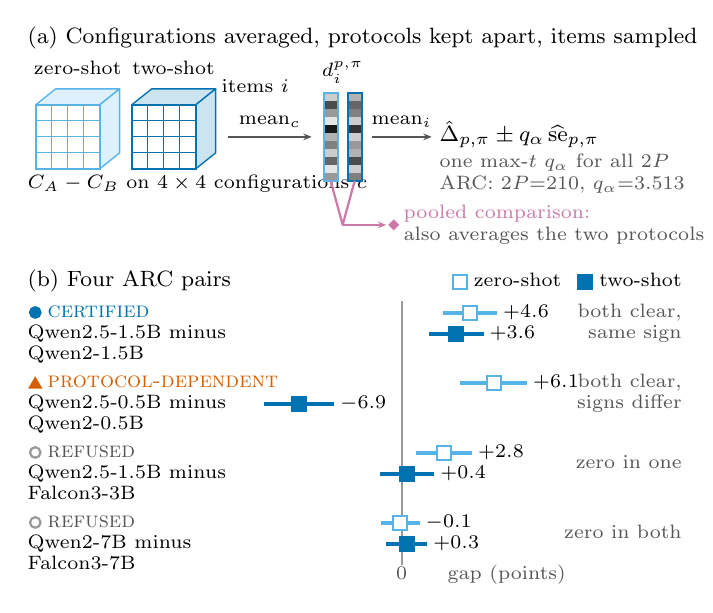
\begin{tikzpicture}[x=1in, y=1in]
\useasboundingbox (0,0) rectangle (3.286,2.786);

%% Panel (a)
\node[L, font=\eig] at (0.00,2.705) {(a) Configurations averaged, protocols kept apart, items sampled};
\node[C] at (0.25,2.55) {zero-shot};
\node[C] at (0.73,2.55) {two-shot};

% configuration blocks: front face 4 x 4 configurations, depth = items
\foreach \xo/\col/\tint in {0.04/ZERO/ZERO20, 0.52/ALG/ALG20}{
  \filldraw[fill=\tint, draw=\col, line width=0.5pt, line join=round]
    (\xo,2.40) -- ({\xo+0.32},2.40) -- ({\xo+0.42},2.48) -- ({\xo+0.10},2.48) -- cycle;
  \filldraw[fill=\tint, draw=\col, line width=0.5pt, line join=round]
    ({\xo+0.32},2.08) -- ({\xo+0.42},2.16) -- ({\xo+0.42},2.48) -- ({\xo+0.32},2.40) -- cycle;
  \fill[white] (\xo,2.08) rectangle ({\xo+0.32},2.40);
  \foreach \k in {1,2,3}{
    \draw[\col, line width=0.3pt] ({\xo+0.08*\k},2.08) -- ({\xo+0.08*\k},2.40);
    \draw[\col, line width=0.3pt] (\xo,{2.08+0.08*\k}) -- ({\xo+0.32},{2.08+0.08*\k});
  }
  \draw[\col, line width=0.8pt] (\xo,2.08) rectangle ({\xo+0.32},2.40);
}
\node[L] at (0.97,2.46) {items $i$};
\node[L] at (0.00,1.98) {$C_A-C_B$ on $4\times4$ configurations $c$};

% arrow 1: mean over configurations
\draw[neutral] (1.00,2.24) -- (1.42,2.24);
\node[C] at (1.21,2.30) {$\operatorname{mean}_c$};

% per-item gap strips, 11 cells of 0.07 x 0.04 in (greys decorative)
\foreach \g [count=\k] in {.2,.7,.4,.1,.9,.3,.5,.2,.6,.1,.4}{
  \pgfmathsetmacro{\pc}{100*\g}
  \fill[black!\pc] (1.48,{2.46-0.04*\k}) rectangle (1.55,{2.50-0.04*\k});
}
\foreach \g [count=\k] in {.3,.6,.5,.2,.8,.2,.4,.3,.7,.2,.5}{
  \pgfmathsetmacro{\pc}{100*\g}
  \fill[black!\pc] (1.60,{2.46-0.04*\k}) rectangle (1.67,{2.50-0.04*\k});
}
\draw[ZERO, line width=0.6pt] (1.48,2.02) rectangle (1.55,2.46);
\draw[ALG, line width=0.6pt] (1.60,2.02) rectangle (1.67,2.46);
\node[C] at (1.575,2.54) {$d^{p,\pi}_i$};

% arrow 2: mean over items, ending on the intervals it produces
\draw[neutral] (1.72,2.24) -- (2.02,2.24);
\node[C] at (1.87,2.30) {$\operatorname{mean}_i$};
\node[L, font=\eig] at (2.06,2.215) {$\hat\Delta_{p,\pi}\pm\qalpha\,\widehat{\mathrm{se}}_{p,\pi}$};
\node[L, text=TEXT2] at (2.06,2.085) {one max-$t$ $\qalpha$ for all $2P$};
\node[L, text=TEXT2] at (2.06,1.975) {ARC: $2P{=}210$, $\qalpha{=}3.513$};

% pooled branch
\draw[POOL, line width=0.8pt, line join=round] (1.515,2.02) -- (1.575,1.80) -- (1.635,2.02);
\draw[POOL, line width=0.8pt, -tip] (1.575,1.80) -- (1.792,1.80);
\pic at (1.83,1.80) {pdia};
\node[L, text=POOL] at (1.88,1.83) {pooled comparison:};
\node[L, text=TEXT2] at (1.88,1.72) {also averages the two protocols};

%% Panel (b)
\node[L, font=\eig] at (0.00,1.49) {(b) Four ARC pairs};
\node[R] (lgt) at (3.27,1.49) {two-shot};
\pic at ([shift={(-0.07,0.025)}]lgt.base west) {tsq};
\node[R] (lgz) at ([xshift=-0.19in]lgt.base west) {zero-shot};
\pic at ([shift={(-0.07,0.025)}]lgz.base west) {zsq};

% gap axis: x 1.12-2.62 spans -10 to +10 points
\draw[zeroline] (1.87,0.10) -- (1.87,1.42);
\node[C, text=TEXT2] at (1.87,0.025) {0};
\node[L, text=TEXT2] at (2.10,0.025) {gap (points)};

% Row 1: certified
\vrow{1.335}{cert}{\Certified}{ALG}{Qwen2.5-1.5B minus}{Qwen2-1.5B}
\interval{1.360}{2.740}{4.553}{6.367}{z}{$+4.6$}
\interval{1.255}{1.842}{3.650}{5.457}{t}{$+3.6$}
\node[R, text=TEXT2] at (3.27,1.335) {both clear,};
\node[R, text=TEXT2] at (3.27,1.230) {same sign};

% Row 2: protocol-dependent
\vrow{0.985}{prot}{\ProtDep}{PLUG}{Qwen2.5-0.5B minus}{Qwen2-0.5B}
\interval{1.010}{3.917}{6.142}{8.367}{z}{$+6.1$}
\interval{0.905}{-9.208}{-6.853}{-4.497}{t}{$-6.9$}
\node[R, text=TEXT2] at (3.27,0.985) {both clear,};
\node[R, text=TEXT2] at (3.27,0.880) {signs differ};

% Row 3: refused, resolved in one protocol
\vrow{0.635}{refu}{\Refused}{TEXT2}{Qwen2.5-1.5B minus}{Falcon3-3B}
\interval{0.660}{0.974}{2.838}{4.703}{z}{$+2.8$}
\interval{0.555}{-1.467}{0.354}{2.175}{t}{$+0.4$}
\node[R, text=TEXT2] at (3.27,0.5825) {zero in one};

% Row 4: refused, unresolved in both protocols
\vrow{0.285}{refu}{\Refused}{TEXT2}{Qwen2-7B minus}{Falcon3-7B}
\interval{0.310}{-1.404}{-0.100}{1.203}{z}{$-0.1$}
\interval{0.205}{-1.050}{0.333}{1.716}{t}{$+0.3$}
\node[R, text=TEXT2] at (3.27,0.2325) {zero in both};

\end{tikzpicture}
\end{document}
